\section{Procedure}

A ramp was propped up using a set of books.
The motion sensor as attached to the top of the ramp, and an initial calibration was taken to determine where a good spot to start recording was.

\begin{figure}[h]

\begin{center}
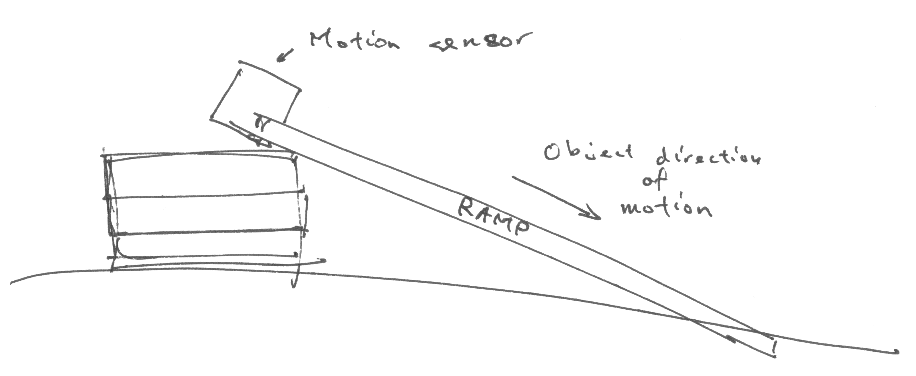
\includegraphics[scale=0.5]{content/fig1}
\end{center}

\caption{The setup of this lab.}

\end{figure}

For each test, the object in question was placed at the starting position, and when the motion sensor was activated, it was released to roll down the board.
The positions and velocities of the objects as they rolled with respect to time were recorded.

For this particular experiment, a wheel, baseball, and orange and blue ball of differing materials, a hollow tube, an aluminum cylinder, and a solid cylinder were used.

